
%% bare_conf.tex
%% V1.4b
%% 2015/08/26
%% by Michael Shell
%% See:
%% http://www.michaelshell.org/
%% for current contact information.
%%
%% This is a skeleton file demonstrating the use of IEEEtran.cls
%% (requires IEEEtran.cls version 1.8b or later) with an IEEE
%% conference paper.
%%
%% Support sites:
%% http://www.michaelshell.org/tex/ieeetran/
%% http://www.ctan.org/pkg/ieeetran
%% and
%% http://www.ieee.org/

%%*************************************************************************
%% Legal Notice:
%% This code is offered as-is without any warranty either expressed or
%% implied; without even the implied warranty of MERCHANTABILITY or
%% FITNESS FOR A PARTICULAR PURPOSE! 
%% User assumes all risk.
%% In no event shall the IEEE or any contributor to this code be liable for
%% any damages or losses, including, but not limited to, incidental,
%% consequential, or any other damages, resulting from the use or misuse
%% of any information contained here.
%%
%% All comments are the opinions of their respective authors and are not
%% necessarily endorsed by the IEEE.
%%
%% This work is distributed under the LaTeX Project Public License (LPPL)
%% ( http://www.latex-project.org/ ) version 1.3, and may be freely used,
%% distributed and modified. A copy of the LPPL, version 1.3, is included
%% in the base LaTeX documentation of all distributions of LaTeX released
%% 2003/12/01 or later.
%% Retain all contribution notices and credits.
%% ** Modified files should be clearly indicated as such, including  **
%% ** renaming them and changing author support contact information. **
%%*************************************************************************


% *** Authors should verify (and, if needed, correct) their LaTeX system  ***
% *** with the testflow diagnostic prior to trusting their LaTeX platform ***
% *** with production work. The IEEE's font choices and paper sizes can   ***
% *** trigger bugs that do not appear when using other class files.       ***                          ***
% The testflow support page is at:
% http://www.michaelshell.org/tex/testflow/



\documentclass[conference]{IEEEtran}
% Some Computer Society conferences also require the compsoc mode option,
% but others use the standard conference format.
%
% If IEEEtran.cls has not been installed into the LaTeX system files,
% manually specify the path to it like:
% \documentclass[conference]{../sty/IEEEtran}





% Some very useful LaTeX packages include:
% (uncomment the ones you want to load)


% *** MISC UTILITY PACKAGES ***
%
%\usepackage{ifpdf}
% Heiko Oberdiek's ifpdf.sty is very useful if you need conditional
% compilation based on whether the output is pdf or dvi.
% usage:
% \ifpdf
%   % pdf code
% \else
%   % dvi code
% \fi
% The latest version of ifpdf.sty can be obtained from:
% http://www.ctan.org/pkg/ifpdf
% Also, note that IEEEtran.cls V1.7 and later provides a builtin
% \ifCLASSINFOpdf conditional that works the same way.
% When switching from latex to pdflatex and vice-versa, the compiler may
% have to be run twice to clear warning/error messages.






% *** CITATION PACKAGES ***
%
\usepackage{cite}
% cite.sty was written by Donald Arseneau
% V1.6 and later of IEEEtran pre-defines the format of the cite.sty package
% \cite{} output to follow that of the IEEE. Loading the cite package will
% result in citation numbers being automatically sorted and properly
% "compressed/ranged". e.g., [1], [9], [2], [7], [5], [6] without using
% cite.sty will become [1], [2], [5]--[7], [9] using cite.sty. cite.sty's
% \cite will automatically add leading space, if needed. Use cite.sty's
% noadjust option (cite.sty V3.8 and later) if you want to turn this off
% such as if a citation ever needs to be enclosed in parenthesis.
% cite.sty is already installed on most LaTeX systems. Be sure and use
% version 5.0 (2009-03-20) and later if using hyperref.sty.
% The latest version can be obtained at:
% http://www.ctan.org/pkg/cite
% The documentation is contained in the cite.sty file itself.






% *** GRAPHICS RELATED PACKAGES ***
%
\ifCLASSINFOpdf
  % \usepackage[pdftex]{graphicx}
  % declare the path(s) where your graphic files are
  % \graphicspath{{../pdf/}{../jpeg/}}
  % and their extensions so you won't have to specify these with
  % every instance of \includegraphics
  % \DeclareGraphicsExtensions{.pdf,.jpeg,.png}
\else
  % or other class option (dvipsone, dvipdf, if not using dvips). graphicx
  % will default to the driver specified in the system graphics.cfg if no
  % driver is specified.
  % \usepackage[dvips]{graphicx}
  % declare the path(s) where your graphic files are
  % \graphicspath{{../eps/}}
  % and their extensions so you won't have to specify these with
  % every instance of \includegraphics
  % \DeclareGraphicsExtensions{.eps}
\fi
% graphicx was written by David Carlisle and Sebastian Rahtz. It is
% required if you want graphics, photos, etc. graphicx.sty is already
% installed on most LaTeX systems. The latest version and documentation
% can be obtained at: 
% http://www.ctan.org/pkg/graphicx
% Another good source of documentation is "Using Imported Graphics in
% LaTeX2e" by Keith Reckdahl which can be found at:
% http://www.ctan.org/pkg/epslatex
%
% latex, and pdflatex in dvi mode, support graphics in encapsulated
% postscript (.eps) format. pdflatex in pdf mode supports graphics
% in .pdf, .jpeg, .png and .mps (metapost) formats. Users should ensure
% that all non-photo figures use a vector format (.eps, .pdf, .mps) and
% not a bitmapped formats (.jpeg, .png). The IEEE frowns on bitmapped formats
% which can result in "jaggedy"/blurry rendering of lines and letters as
% well as large increases in file sizes.
%
% You can find documentation about the pdfTeX application at:
% http://www.tug.org/applications/pdftex





% *** MATH PACKAGES ***
%
\usepackage{bm}
\usepackage{amsmath}
\usepackage{graphicx}
\graphicspath{{fig/}}
\usepackage{caption}
% A popular package from the American Mathematical Society that provides
% many useful and powerful commands for dealing with mathematics.
%
% Note that the amsmath package sets \interdisplaylinepenalty to 10000
% thus preventing page breaks from occurring within multiline equations. Use:
%\interdisplaylinepenalty=2500
% after loading amsmath to restore such page breaks as IEEEtran.cls normally
% does. amsmath.sty is already installed on most LaTeX systems. The latest
% version and documentation can be obtained at:
% http://www.ctan.org/pkg/amsmath





% *** SPECIALIZED LIST PACKAGES ***
%
%\usepackage{algorithmic}
% algorithmic.sty was written by Peter Williams and Rogerio Brito.
% This package provides an algorithmic environment fo describing algorithms.
% You can use the algorithmic environment in-text or within a figure
% environment to provide for a floating algorithm. Do NOT use the algorithm
% floating environment provided by algorithm.sty (by the same authors) or
% algorithm2e.sty (by Christophe Fiorio) as the IEEE does not use dedicated
% algorithm float types and packages that provide these will not provide
% correct IEEE style captions. The latest version and documentation of
% algorithmic.sty can be obtained at:
% http://www.ctan.org/pkg/algorithms
% Also of interest may be the (relatively newer and more customizable)
% algorithmicx.sty package by Szasz Janos:
% http://www.ctan.org/pkg/algorithmicx




% *** ALIGNMENT PACKAGES ***
%
%\usepackage{array}
% Frank Mittelbach's and David Carlisle's array.sty patches and improves
% the standard LaTeX2e array and tabular environments to provide better
% appearance and additional user controls. As the default LaTeX2e table
% generation code is lacking to the point of almost being broken with
% respect to the quality of the end results, all users are strongly
% advised to use an enhanced (at the very least that provided by array.sty)
% set of table tools. array.sty is already installed on most systems. The
% latest version and documentation can be obtained at:
% http://www.ctan.org/pkg/array


% IEEEtran contains the IEEEeqnarray family of commands that can be used to
% generate multiline equations as well as matrices, tables, etc., of high
% quality.




% *** SUBFIGURE PACKAGES ***
%\ifCLASSOPTIONcompsoc
%  \usepackage[caption=false,font=normalsize,labelfont=sf,textfont=sf]{subfig}
%\else
%  \usepackage[caption=false,font=footnotesize]{subfig}
%\fi
% subfig.sty, written by Steven Douglas Cochran, is the modern replacement
% for subfigure.sty, the latter of which is no longer maintained and is
% incompatible with some LaTeX packages including fixltx2e. However,
% subfig.sty requires and automatically loads Axel Sommerfeldt's caption.sty
% which will override IEEEtran.cls' handling of captions and this will result
% in non-IEEE style figure/table captions. To prevent this problem, be sure
% and invoke subfig.sty's "caption=false" package option (available since
% subfig.sty version 1.3, 2005/06/28) as this is will preserve IEEEtran.cls
% handling of captions.
% Note that the Computer Society format requires a larger sans serif font
% than the serif footnote size font used in traditional IEEE formatting
% and thus the need to invoke different subfig.sty package options depending
% on whether compsoc mode has been enabled.
%
% The latest version and documentation of subfig.sty can be obtained at:
% http://www.ctan.org/pkg/subfig




% *** FLOAT PACKAGES ***
%
%\usepackage{fixltx2e}
% fixltx2e, the successor to the earlier fix2col.sty, was written by
% Frank Mittelbach and David Carlisle. This package corrects a few problems
% in the LaTeX2e kernel, the most notable of which is that in current
% LaTeX2e releases, the ordering of single and double column floats is not
% guaranteed to be preserved. Thus, an unpatched LaTeX2e can allow a
% single column figure to be placed prior to an earlier double column
% figure.
% Be aware that LaTeX2e kernels dated 2015 and later have fixltx2e.sty's
% corrections already built into the system in which case a warning will
% be issued if an attempt is made to load fixltx2e.sty as it is no longer
% needed.
% The latest version and documentation can be found at:
% http://www.ctan.org/pkg/fixltx2e


%\usepackage{stfloats}
% stfloats.sty was written by Sigitas Tolusis. This package gives LaTeX2e
% the ability to do double column floats at the bottom of the page as well
% as the top. (e.g., "\begin{figure*}[!b]" is not normally possible in
% LaTeX2e). It also provides a command:
%\fnbelowfloat
% to enable the placement of footnotes below bottom floats (the standard
% LaTeX2e kernel puts them above bottom floats). This is an invasive package
% which rewrites many portions of the LaTeX2e float routines. It may not work
% with other packages that modify the LaTeX2e float routines. The latest
% version and documentation can be obtained at:
% http://www.ctan.org/pkg/stfloats
% Do not use the stfloats baselinefloat ability as the IEEE does not allow
% \baselineskip to stretch. Authors submitting work to the IEEE should note
% that the IEEE rarely uses double column equations and that authors should try
% to avoid such use. Do not be tempted to use the cuted.sty or midfloat.sty
% packages (also by Sigitas Tolusis) as the IEEE does not format its papers in
% such ways.
% Do not attempt to use stfloats with fixltx2e as they are incompatible.
% Instead, use Morten Hogholm'a dblfloatfix which combines the features
% of both fixltx2e and stfloats:
%
% \usepackage{dblfloatfix}
% The latest version can be found at:
% http://www.ctan.org/pkg/dblfloatfix




% *** PDF, URL AND HYPERLINK PACKAGES ***
%
%\usepackage{url}
% url.sty was written by Donald Arseneau. It provides better support for
% handling and breaking URLs. url.sty is already installed on most LaTeX
% systems. The latest version and documentation can be obtained at:
% http://www.ctan.org/pkg/url
% Basically, \url{my_url_here}.




% *** Do not adjust lengths that control margins, column widths, etc. ***
% *** Do not use packages that alter fonts (such as pslatex).         ***
% There should be no need to do such things with IEEEtran.cls V1.6 and later.
% (Unless specifically asked to do so by the journal or conference you plan
% to submit to, of course. )


% correct bad hyphenation here
\hyphenation{op-tical net-works semi-conduc-tor}


\begin{document}
%
% paper title
% Titles are generally capitalized except for words such as a, an, and, as,
% at, but, by, for, in, nor, of, on, or, the, to and up, which are usually
% not capitalized unless they are the first or last word of the title.
% Linebreaks \\ can be used within to get better formatting as desired.
% Do not put math or special symbols in the title.
\title{A Survey of Four Popular Techniques \\ used in Face Recognition}


% author names and affiliations
% use a multiple column layout for up to three different
% affiliations
\author{
	\IEEEauthorblockN{Yi Han}
	\IEEEauthorblockA{Department of Electrical and\\Computer Engineering\\
	Rutgers, the State University of New Jersy}
}

% conference papers do not typically use \thanks and this command
% is locked out in conference mode. If really needed, such as for
% the acknowledgment of grants, issue a \IEEEoverridecommandlockouts
% after \documentclass

% for over three affiliations, or if they all won't fit within the width
% of the page, use this alternative format:
% 
%\author{\IEEEauthorblockN{Michael Shell\IEEEauthorrefmark{1},
%Homer Simpson\IEEEauthorrefmark{2},
%James Kirk\IEEEauthorrefmark{3}, 
%Montgomery Scott\IEEEauthorrefmark{3} and
%Eldon Tyrell\IEEEauthorrefmark{4}}
%\IEEEauthorblockA{\IEEEauthorrefmark{1}School of Electrical and Computer Engineering\\
%Georgia Institute of Technology,
%Atlanta, Georgia 30332--0250\\ Email: see http://www.michaelshell.org/contact.html}
%\IEEEauthorblockA{\IEEEauthorrefmark{2}Twentieth Century Fox, Springfield, USA\\
%Email: homer@thesimpsons.com}
%\IEEEauthorblockA{\IEEEauthorrefmark{3}Starfleet Academy, San Francisco, California 96678-2391\\
%Telephone: (800) 555--1212, Fax: (888) 555--1212}
%\IEEEauthorblockA{\IEEEauthorrefmark{4}Tyrell Inc., 123 Replicant Street, Los Angeles, California 90210--4321}}




% use for special paper notices
%\IEEEspecialpapernotice{(Invited Paper)}




% make the title area
\maketitle

% As a general rule, do not put math, special symbols or citations
% in the abstract
\begin{abstract}
In this paper we explored four popular techniques used in face recognition. Eigenface and Fisherface are well-known subspace methods for dimension reduction, Support Vector Machine(SVM) is a widely used classifier over the past decade. We also looked into a relatively young but very powerful method, Sparse Representation-based Classification(SRC). Experiments and comparisons were made among these four techniques. 
\end{abstract}

% no keywords




% For peer review papers, you can put extra information on the cover
% page as needed:
% \ifCLASSOPTIONpeerreview
% \begin{center} \bfseries EDICS Category: 3-BBND \end{center}
% \fi
%
% For peerreview papers, this IEEEtran command inserts a page break and
% creates the second title. It will be ignored for other modes.
\IEEEpeerreviewmaketitle



\section{Introduction}
Face recognition is a widely and deeply studied topic in computer vision, it has a number of applications including surveillance cameras, secure authentication and human/computer interface etc. Over the past two decades enormous effect has been put in the area, a great many algorithms and their variations have been proposed to deal with challenges in face recognition such as illumination, facial expression and occlusion etc. 

In this paper, we discussed four face recognition techniques which are of great importance and been used in real-world applications. Eigenface and Fisherface are all subspace methods, they seek a subspace of the feature space, where projection of feature vectors onto the subspace retain high variance while at the same time reduce computation complexity significantly. Eigenface treats image samples as observations of a random vector, first tries to make random variables in the vector uncorrelated with each other by diagonalizing the covariance matrix with its eigenvectors, it's like fitting the data with a multivariate Gaussian distribution, or in other words, an ellipsoid. it then chooses a subspace spanned by part of the eigenvectors which preserves most of the variance, the process can be viewed as finding a cross section of the ellipsoid through origin which has longer axises, the length of the axises are just eigenvalues of the covariance matrix. Eigenface scatters all the samples in the subspace,  without taking class information, which is vital for classification, into consideration, so Eigenface is kind of mixing data together, while it's advantage is at computation complexity: by projecting all data into the subspace, feature length is significantly reduced, so is computing time. Fisherface however, managed to incorporate class information into the object. It tries to maximize between class scatter while at the same time minimize within class scatter. In this sense, samples are clustered according to the class information, thus can be easily classified. Eigenface and Fisherface are actually feature extraction methods, the try to obtain an compact representation of the image. To deal with the recognition task, classifiers are needed.

Support Vector Machine(SVM) is probably the dominant classifier in the last two decades. SVM tries to learn a hyperplane between two different classes of data, which maximize the margin between the plane supported by support vectors of each class and the hyperplane. The hyperplane can be viewed as a decision function thus data from different classes can be well separated. In the linearly inseparable case, kernel functions are involved to map data to a higher, linear separable dimension. However, experimental results shows that SVM relies heavily on choices of parameters and size of training set, improper parameters or small training set may results in unacceptable classification accuracy. Thus a cross validation technique is required to search for the best parameters. Sparse Representation-based classification(SRC) is a relatively young but promising method been studied over the past few years. SRC borrowed the idea of sparse representation from compressed sensing in signal processing field, which represents each query image with samples in the training set, or in other words, transforms each image into the space spanned by samples in the training set. The result vector will only have large coefficients in the entries corresponding to training images of the same class, thus it's very sparse. The process can be viewed as solving an underdetermined linear system of equations, thus the solution is not unique, seeking for the sparest solution, we can get the best representation of each query image corresponding to all images in the training set. Then residual comparisons between original images and the image reconstructed by their sparse representations are made to determine the classification results. Experimental result shows that SRC is very power full even with a training set of very small size.

We explored the concepts and theories of these four techniques, tried to look into their advantages as well as drawbacks. We tested these methods on the extended YaleB dataset, looked into the influence of some parameters. The remaining content of the paper is organized as follow: In section 2, we explained the theories of these four methods; In section 3, we gave our experimental results and analysis; In section 4, we draw our conclusions and propose some challenges that might be improved in further studies.


\section{Methods}
\subsection{Eigenface}
Eigenface depends mainly on Principal Components Analysis(PCA). PCA diagonalizes the covariance matrix of a set of samples which is assumed to be generated from the a same probability distribution by its eigenvectors. These eigenvectors are called the principal components of the data. The diagonal entries of the result matrix is the variance of each random variable in the distribution. it can be shown that when arranged in descending order, only a few variance in the beginning can take contain nearly all the information.

Suppose we have a set of samples $\bm{x}_i,\, i=1,...,n$, the covariance matrix $S$ is computed as follow
\begin{equation}
	S= \sum_{i=1}^{n}(\bm{x}_i-\bm{\mu})(\bm{x}_i-\bm{\mu})^T
\end{equation}
where $\bm{\mu}$ is the sample mean of all the data.
if we put all the data in a matrix:
\begin{equation}
	B = 
	\begin{bmatrix}
	\bm{x}_1-\bm{\mu}\quad\bm{x}_2-\bm{\mu}\quad ...\quad\bm{x}_n-\bm{\mu}
	\end{bmatrix}
\end{equation}
the equation can be written as follow
\begin{equation}
	S = BB^T
\end{equation}
We seek a projection matrix $W$, which transforms all samples to a space spanned by the column of it
\begin{equation}
	\bm{y} = W^T\bm{x}
\end{equation}
if we assume $W$ to be eigenvectors of S and compute the covariance matrix $D$ of the new random vector $y$, we can easily find out that its just the diagonal matrix mentioned above:
\begin{equation}
	D=(W^T\bm{x})(W^T\bm{x})^T = W^TSW
\end{equation} 
thus columns of $W$ are the principle components, or eigenfaces if we reshape them to be a image(Fig. \ref{eigenface}). By diagonalizing the covariance matrix $S$, we make the data uncorrelated. Note that the \textit{Total Variance} of the data, that is sum of variance within each dimension, remains unchanged before and after diagonalization since $tr(S) = \sum \lambda_i$, where $\lambda_i$ are eigenvalues of $S$.

As mentioned above, most variance of the data is contained by a few biggest principal components, thus to achieve better computation efficiency, we take only these big principal components to construct the projection matrix. In an optimization perspective, this can be expressed as
\begin{equation}
	W_{opt}=\arg\: \max_W |W^TSW|
\end{equation}
where $W_{opt}$ is a $n\times k$ matrix where $n$ is the dimension of the data and $k$ is the number of principal components we want to take. The solution of this optimization problem is shown to be just taking eigenvectors corresponding to largest $k$ eigenvalues of $S$. Experiments shows that less then 3\% of the principal components contains more than 90\% of the variance, thus computing time in further classification tasks is significantly reduced.
\begin{figure}[htbp]
	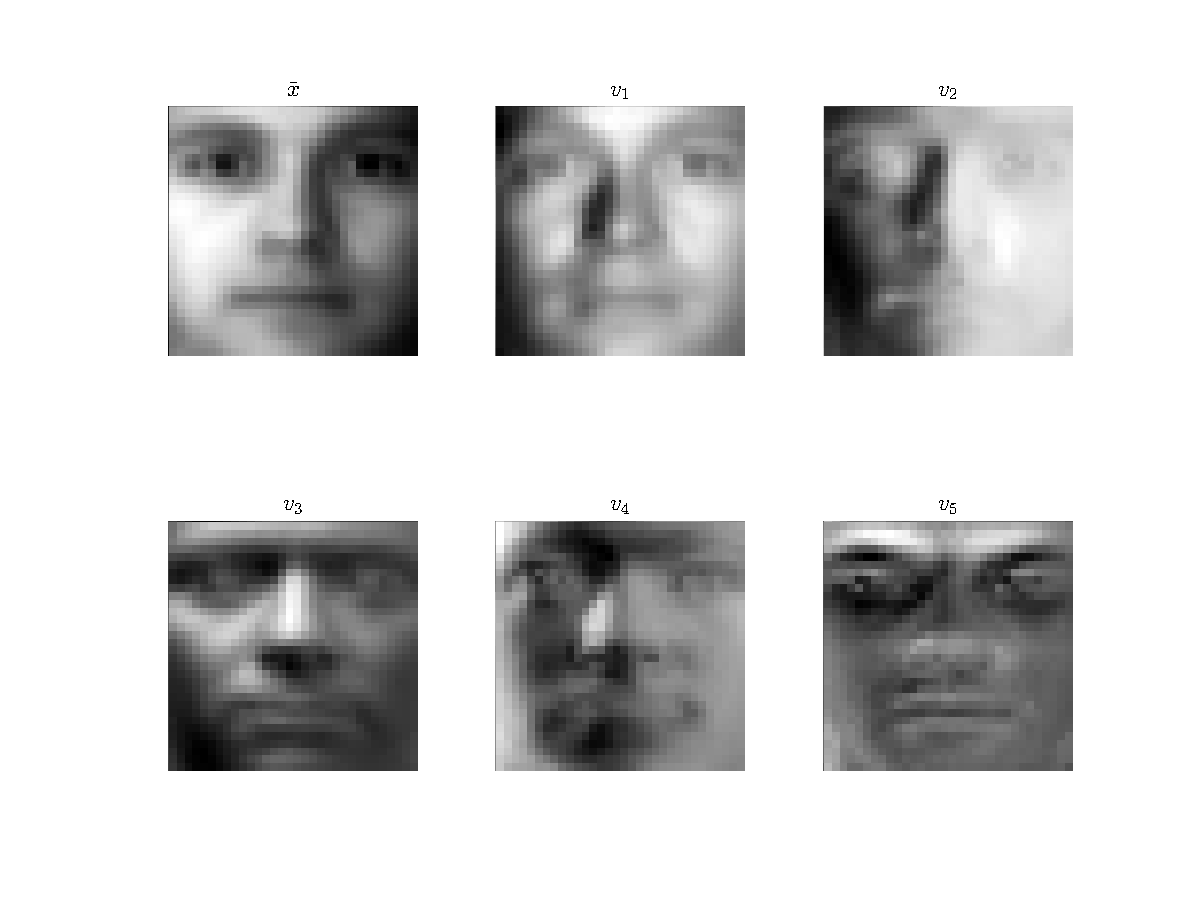
\includegraphics[width=0.5\textwidth]{eigenface}
	\caption{Visualization of eigenfaces. Largest three eigenvectors correspond to variation due to lighting.}
	\label{eigenface}
\end{figure}

It is almost always the case in face recognition task that the dimension of each sample is very large, covariance matrix $S$ therefore is huge. Doing eigenvalue decomposition on such matrices is time consuming. However, if we look at the definition of the covariance matrix, $S=BB^T$, and the key idea in Singular Value Decomposition(SVD)
\begin{equation}
	 \sigma_i \bm{v_i}=B\bm{u_i}
\end{equation}
where $\bm{u_i}$ is eigenvectors of $A^TA$ while $\bm{v_i}$ is eigenvectors of $AA^T$, and in our case $\sigma_i$ is eigenvalues of $S$, we can easily find out that by doing eigenvalue decomposition on $B^TB$ instead of $BB^T$, and compute computing eigenvalues of $S$ by $\bm{v_i}=B\bm{u_i}/\sigma_i$, we can reduce the size of the covariance matrix from dimension of samples to number of samples in the training set, in most case this is a significant reduction.

The main drawback of Eigenface is none other than the way it projects samples: Eigenface did not take class information into consideration, it tries to maximize the scatter of all samples while to make data more discriminative, we want within class scatter to be small. discarding such this, Eigenface is kind of preserving unwanted information which corresponding to illumination changes between images from the same class\cite{adini1997face}(illumination changes can be viewed as a translation in the sample space, which separates samples within the same class). Thus data are not well clustered, or even smeared together, making them no longer linearly separable. Therefore, the Main accomplishment of Eigenface is reducing the computation complexity, not improving the discriminative power, we can not expect a higher classification result since the projection process along is losing variances. By discarding the first three principal components, we can expect a better performance since the influence of illumination has been removed\cite{belhumeur1997eigenfaces}. As mentioned above, PCA is trying to fit the data with a ellipsoid, thus Eigenface works well on data with Gaussian distribution, for data in other distribution format, the result may not be that good.
\subsection{Fisherface}
Similar as Eigenface, the Fisherface is also trying to project data onto a subspace. However, unlike Eigenface, which treat every data sample uniformly, Fisherface takes advantage of class information. Thus a better discrimination is achieved between different classes. It's like a supervised way of clustering the data, and consequently classification is simplified.

The Within-class scatter can be defined as
\begin{equation}
	S_W=\sum_{ij}(\bm{x}_{ij}-\bm{\mu}_i)(\bm{x}_{ij}-\bm{\mu}_i)^T
\end{equation}
and the total scatter, as defined in last section, is
\begin{equation}
	S_T=\sum_{ij}(\bm{x}_{ij}-\bm{\mu})(\bm{x}_{ij}-\bm{\mu})^T
\end{equation}
according to these two equation, we can derivate the between class by subtracting within-class from total scatter:
\begin{equation}
	\begin{split}
		S_B 
		& =\sum_{ij}[(\bm{\mu}_i-\bm{\mu})+(\bm{x}_{ij}-\bm{\mu}_i)][(\bm{\mu}_i-\bm{\mu})+(\bm{x}_{ij}-\bm{\mu}_i]^T \\
		& =\sum_{ij}(\bm{\mu}_i-\bm{\mu})(\bm{\mu}_i-\bm{\mu})^T+\sum_{ij}(\bm{x}_{ij}-\bm{\mu}_i)(\bm{x}_{ij}-\bm{\mu}_i)^T \\
		&
		\quad+\sum_{ij}(\bm{\mu}_i-\bm{\mu})(\bm{x}_{ij}-\bm{\mu}_i)^T+\sum_{ij}(\bm{\mu}_i-\bm{\mu})(\bm{x}_{ij}-\bm{\mu}_i)^T
	\end{split}
\end{equation}
for the last two terms in the above equation,
\begin{equation}
	\begin{split}
	&
	\quad\sum_{ij}(\bm{\mu}_i-\bm{\mu})(\bm{x}_{ij}-\bm{\mu}_i)^T \\
	&
	=\sum_{j}(\bm{x}_{ij}-\bm{\mu}_i)\sum_{i}(\bm{\mu}_i-\bm{\mu}) \\
	&
	=(\sum_{j}\bm{x}_{ij}-\sum_{j}\bm{\mu}_i)\sum_{i}(\bm{\mu}_i-\bm{\mu})^T \\
	&
	=0\times\sum_{i}(\bm{\mu}_i-\bm{\mu}) \\
	&=0
	\end{split}
\end{equation}
the other term can be computed in the same way. Also,
\begin{equation}
	\begin{split}
		&
		\quad\sum_{ij}(\bm{\mu}_i-\bm{\mu})(\bm{\mu}_i-\bm{\mu})^T \\
		&
		=\sum_{i=1}^{c}\sum_{j=1}^{N_i}(\bm{\mu}_i-\bm{\mu})(\bm{\mu}_i-\bm{\mu})^T \\
		&
		=\sum_{i=1}^{c}N_i(\bm{\mu}_i-\bm{\mu})(\bm{\mu}_i-\bm{\mu})^T
	\end{split}
\end{equation}
thus 
\begin{equation}
	\begin{split}
		S_T
		&
		=\sum_{ij}(\bm{\mu}_i-\bm{\mu})(\bm{\mu}_i-\bm{\mu})^T+\sum_{ij}(\bm{x}_{ij}-\bm{\mu}_i)(\bm{x}_{ij}-\bm{\mu}_i)^T \\
		&
		=\sum_{i=1}^{c}N_i(\bm{\mu}_i-\bm{\mu})(\bm{\mu}_i-\bm{\mu})^T+S_W
	\end{split}
\end{equation}
the total scatter can be split into within-class scatter and between-class scatter, thus the between-class scatter is defined as
\begin{equation}
	S_B=\sum_{i=1}^{c}N_i(\bm{\mu}_i-\bm{\mu})(\bm{\mu}_i-\bm{\mu})^T
\end{equation}
However, the above way of defining between-class scatter in unbalanced, classes with larger number of samples will dominant the result. To deal with this, we might consider a balanced formula
\begin{equation}
	S_B^*=\bar{n}\sum_{i}(\bm{\mu}_i-\bm{\mu}^*)(\bm{\mu}_i-\bm{\mu}^*)^T
\end{equation}
where $\bar{n}=\sum_{i}N_i/c$ is averaging the class size, $\bm{\mu}^*=\sum_i\bm{\mu}_i/c$ is averaging the class centres. $S_T^*$ and $S_W^*$ can be defined in a similar way. Note that if each class contains same number of training samples, these two formula coincide.

One way from a optimization perspective of expressing the concept of maximizing the between-class scatter while at the same time minimizing the within-class scatter is
\begin{equation}
	W_opt=\arg\,\max_{W}\frac{|W^TS_BW|}{|W^TS_WW|}
\end{equation}
it is worth noticing that the object function is invariant to scaling of $W: W\rightarrow \alpha W$, thus we can alway set the denominator to 1, convert the optimization problem to
\begin{equation}
	\begin{split}
		\arg\,\max_{W}\quad&-\frac{1}{2}WTS_BW \\  \mathrm{s.t.}  \quad &W^TS_BW=1
	\end{split}
\end{equation}
the lagrangian of the problem is
\begin{equation}
	L_p=-\frac{1}{2}W^TS_BW+\frac{1}{2}\lambda(W^TS_WW-1)
\end{equation}
note that both $\frac{1}{2}$ are added for convenience. Set the first orer derivative to zero, we get
\begin{equation}
	S_BW=\lambda S_WW
	\label{gen}
\end{equation}
Left multiply $W^T$ on both side of the equation, and solve for $\lambda$, we get
\begin{equation}
	\lambda=\frac{|W^TS_BW|}{|W^TS_WW|}
\end{equation}
It's just the object function of the original optimization problem. Eq. \ref{gen} is a generalized eigenvalue problem, thus solving the optimization problem is equal to find the eigenvectors corresponding to the largest $k$ eigenvalues of the generalized eigenvalue problem if we restrict the number of column of $W$ to be $k$.

The maximum rank of $S_B$ is $c-1$
\begin{equation}
	\begin{split}
		&
		\quad\; rank(\sum_{i}(\bm{\bm{\mu}}_i -\bm{\mu})(\bm{\bm{\mu}}_i -\bm{\mu})^T) \\
		&=rank(\sum_{i}\bm{\bm{\mu}}_i\bm{\bm{\mu}}_i^T)-rank(\sum_{i}\bm{\bm{\mu}}_i\bm{\mu}^T)- \\
		&
		\quad\;rank(\sum_{i}\bm{\mu}\bm{\bm{\mu}}_i^T)+rank(\sum_{i}\bm{\mu}\bm{\mu}^T) \\
		&
		= c-1-1+1 \\
		&
		=c-1
	\end{split}
\end{equation}
Thus the upper bound of number of eigenvalues of the generalized eigenvalue problem is $c-1$, which means information is well concentrated in a few dimensions.

Most cases in face recognition, due to insufficiency of training samples, we are confronted with the difficulty that the within-class scatter $S_W$ is singular(rank at most be $N-c$) due to insufficiency of training samples compared to number of image pixels. Therefore the generalized eigenvalue problem cannot be solve by simply computing the inverse of $S_W$, then doing eigenvalue decomposition on $S_W^{-1}S_B$. To deal with this problem, we usually do a PCA first to reduce to dimension of the samples, then the optimal projection matrix can be written as
\begin{equation}
	W_{opt}=W_{pca}W_{lda}
\end{equation}
\subsection{Support Vector Machine}
Support Vector Machine is perhaps the most popular classification tool in the past twenty years, before Neural Network stages its comeback. 
\subsubsection{Linear classification}

In the simplest linearly seprable case, SVM tries to learn a hyperplane
\begin{equation}
	f(\bm{x})=\bm{w}^T\bm{x}+b
\end{equation}
that serves as a decision plane, which separate samples in two different classes. SVM belong to the class of maximum margin classifiers\cite{heisele2001face}. It looks for the hyperplane that maximize the margin between the support plane of each class with itself. The primal problem model can be expressed as
\begin{equation}
	\begin{split}
		\min_{\bm{w},b,\xi} \quad  &  \frac{1}{2}\bm{w}^T\bm{w}+C\sum_{i=1}^{l}\xi_i \\
		\textrm{s.t.} \quad & y_i(\bm{w}^Tx_i+b)\geq 1-\xi_i \\
		& \xi_i \geq 0,\; i=1,...l.
	\end{split}
\end{equation}
where the latter term is added for tolerance of error, or soft-margin to be precise\cite{chang2011libsvm}. The dual problem is
\begin{equation}
	\begin{split}
		\min_{\bm{w},b,\xi} \quad  &  \frac{1}{2}\bm{\alpha}^TQ\bm{\alpha}-\bf{1}^T\bm{\alpha} \\
		\textrm{s.t.} \quad & \bm{y}^T\bm{\alpha}=0 \\
		& 0 \leq \alpha_i \leq C,\; i=1,...l.
	\end{split}
\end{equation}
where $Q$ is the $l\times l$ positive semidefinite matrix, $Q_{ij}=y_iy_j\langle\bm{x}_i,\bm{x}_j\rangle$. The dual problem can be derivated from the primal problem by apply the method of Lagrange multipliers to combine the object function and the constraints and set its 1st order derivative with respect to $\bm{w}$ and $b$ to 0.

While most of the techniques used to train classifiers are based on the idea of minimizing the training error, which is called \textit{empirical risk}, SVM operate on another induction principle, called \textit{structural risk minimization},which minimizes an upper bound on the generalization error.
\subsubsection{Kernal SVM}
The idea of the decision plane can be easily extended to higher dimensions when the data is not linearly separable. By mapping the data to a higher dimensional space $\bm{z}=\phi(\bm{x}_i)$, a hyperplane may be found to separate the data. Thank to kernel methods, we don't have to compute the mapping for each training samples but compute the kernel function instead
\begin{equation}
	\kappa(\bm{x}_i,\bm{x}_j)=\phi(\bm{x}_i)\phi(\bm{x}_j)
\end{equation}
Consequently the hyperplane, or the decision function can be expressed as 
\begin{equation}
	f(\bm{x})= \sum_{i=1}^{n}\alpha_iy_i\kappa(\bm{x}_i,\bm{x}_j)+b
\end{equation}
Commonly used kernel functions are polynomial, radial basis function, sigmoid. 
\subsubsection{Multi-class classification}
For multi-class classification task, either one-vs-one or one-vs-all approach is applied\cite{heisele2001face}. In one-vs-one way totally $c(c-1)/2$ SVMs are trained, each separate a pair of classes if we assume the number of classes to be $c$. In one-vs-all way only c SVMs are trained, however it may suffer from the problem of imbalanced training set.
\subsection{Sparse Representation-based Classification}
Sparse Representation-based Classification(SRC) is a relatively young method first proposed by Wright in 2009\cite{wright2009robust}. However, the idea of sparse representation is not new at all, in fields such as signal processing, the concept of sparse is also broadly studied. 
\subsubsection{Sparse Representation}
The key idea of sparse representation is represent query images with all the samples in the training set, this is equal to solving the following linear system of equations
\begin{equation}
	\bm{y}=A\bm{x}
\end{equation}
where $\bm{y}$ are query images and $A$ is the matrix columns of who is training samples, $\bm{x}_0$ is the sparse representation we want to obtain. The linear system of equations is usually underdetermined, thus unique solution cannot be achieved. Instead, we seek the sparsest solution using $L_0$-minimization
\begin{equation}
	\begin{split}
		\arg \min_{\bm{x}}\quad&||\bm{x}||_0\\
		\textrm{s.t.}\quad & A\bm{x}=\bm{y}
	\end{split}
\end{equation}
However, this problem is NP-hard\cite{amaldi1998approximability}. Theory in compressed sensing shows that if the solution is sufficiently sparse, $L_0$-minimization can be approximated by $L_1$-minimization\cite{wangrobust}
\begin{equation}
\begin{split}
\arg \min_{\bm{x}}\quad&||\bm{x}||_1\\
\textrm{s.t.}\quad & A\bm{x}=\bm{y}
\end{split}
\end{equation}
The reason $L_2$-minimization is not applied is that solutions from $L_2$-minimization are not sparse at all\cite{wright2009robust}, thus response of the system corresponding to each query image is not well concentrated around the class it belongs to.

Sparse representation is discriminative naturally, as it could select the subset of base vectors which express the input signal most concentrated and automatically reject other less concentrated representation\cite{wangrobust}.
\subsubsection{Classification on Sparse Representation}
For classification task, we simple reconstruct the image corresponding to each class of train samples, compute the residual of it between the real query image. it's intuitive that reconstruction with the smallest residual is most likely to be the true class the query image belongs to. The process can be expressed as follow
\begin{equation}
	\min_{i}r_i(\bm{y})=||\bm{y}-A\gamma_i(\bm{\hat{x}})||_2
\end{equation} 
where $\gamma_i$ is a function that selects the coefficients within the $i$th class.

Compared with other popular classification methods such as Nearest Neighbour and SVM, SRC classifies test image based on all possible support within the training set\cite{wright2009robust}, while Nearest Neighbour uses only one and SVM uses those on the support plane, thus is expected to have preciser description of query images.

One more thing worth noticing is that once the sparsity is harnessed, the choice of different features is no longer critical\cite{wangrobust}.
\section{Experimental Results}
In this section, we apply the aforementioned four methods to the extended YaleB dataset, which contains 38 individuals, each individual have around 60 samples. We simply vectorize each image to form a description. We first look into the overall performance of each method. Then we vary the number of principal components in Eigenface and Fisherface, try to evaluate it's influence on the classification result. Finally, we looked into the influence of size of training set, make comparison to different methods and strategies.

\subsection{Overall Performance}

Here we present the best classification result of each method we can reach.We picked 50 training sample per class, and do the testing on the rest, each experiment is repeated 5 times for stability. For the first two subspace method, we applied both a Nearest Neighbour(NN) classifier\cite{scikit-learn} and SVM\cite{chang2011libsvm} to achieve the accuracy, for SVM, a cross-validation
process is performed to guarantee a good result, for SRC, we did nothing, just let it run, but the result seems to defeat any other methods.
\begin{center}
	\captionof{table}{Classification results over different methods.}
	\begin{tabular}{|c c c|} 
		\hline
		Eigenface+NN & Fisherface+NN & SVM  \\ 
		\hline
		 81.13\% & 95.06\% & 94.94\%  \\  
		\hline
		Eigenface+SVM & Fisherface+SVM &  SRC  \\   
		\hline
		79.56\% & 94.36\% &  99.03\%  \\
		\hline
	\end{tabular}
\end{center}

Eigenface achieves the lowest accuracy compared to other methods, no matter simple Nearest Neighbour classifier or advanced SVM is applied, this coincides with our deduction that PCA reduces discriminative power between different classes, smears all samples together, thus followed by a SVM classifier, which seeks a hyperplane that linearly separate the data, is worse than simply finding the nearest neighbour.  Fisherface shows similar results on both NN and SVM, and the classification accuracy is satisfying. As mentioned above, Fisherface makes use of class label information, thus gains better discrimination, it like shaping the data, making them clustered. SVM along obtains similar results, however, without dimension reduction, the computation complexity is high, especially a cross validation process is applied. Moreover, the cross validation is necessary to obtain a reasonable result, casual choice of some parameters may results in an unacceptable classification accuracy. SRC shows surprisingly high accuracy, it's nearly $100\%$. SRC seeks all possible support for the representation of query images, owe to the sparsity of the representation, the coefficients is highly concentrated, thus each images is well described and discrimination between different classes is obvious. However, In our experiment, as the size of the training size increased, the computing time of SRC rises significantly even under a parallel computing setup, thus further study might need to be conducted to fit it into a real-world application.

\subsection{Influence of k}
In this experiment we test the influence of number of principal components we pick for the project matrix on the classification result. We set the training sample per class to be 50, and again each run of experiment is repeated 5 times for the stability of the results.
\begin{figure}[htbp]
	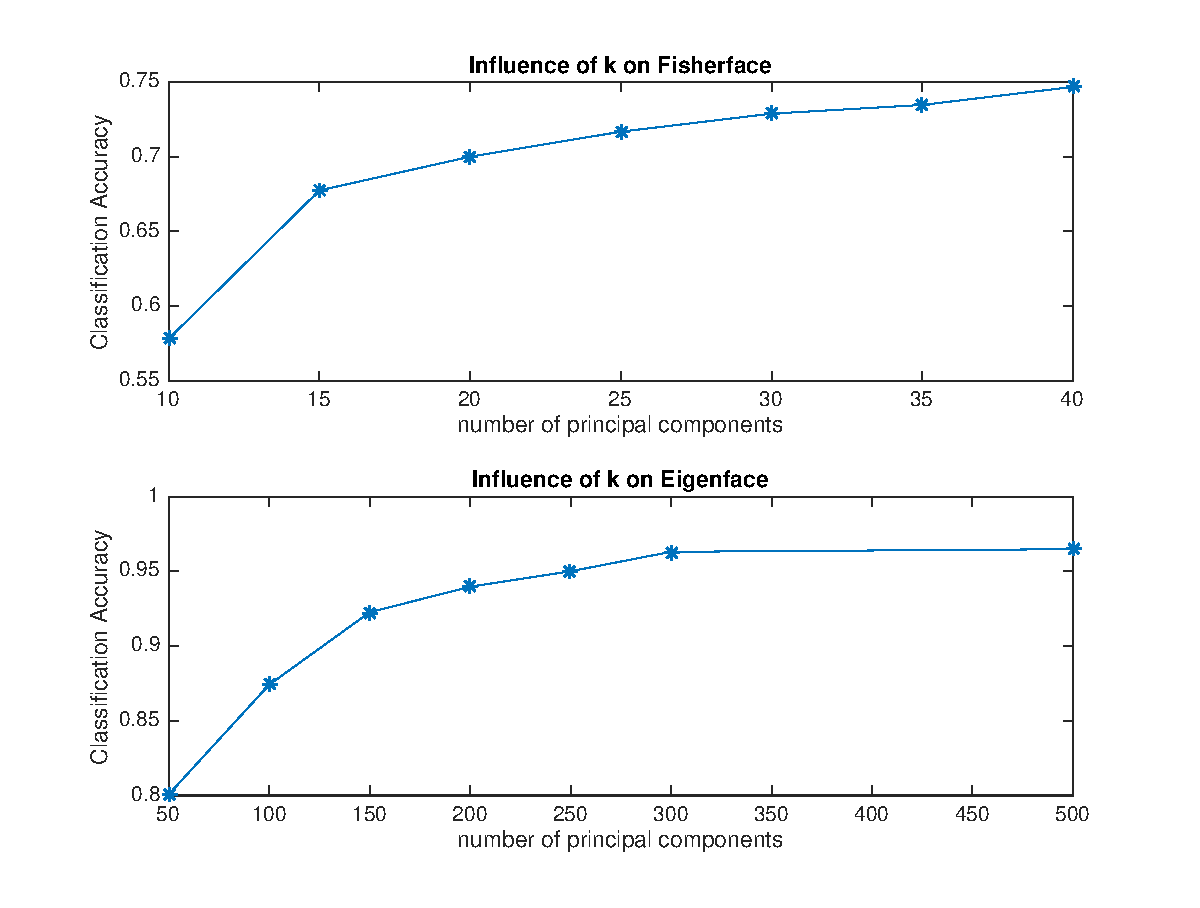
\includegraphics[width=0.5\textwidth]{infk}
	\caption{Influence of number of principal components. A small percentage of principal components is enough to obtain a satisfying classification accuracy}
	\label{infk}
\end{figure}
As shown in Fig. \ref{infk}, both Eigenface and Fisherface achieve steady results after the number of principal components rises rises. Only a small rise is enough to obtain steady results. Thus by project data onto the subspace of such small dimension, the computation is significantly reduced comparing with the original feature of all image pixels.
\subsection{Influence of training set size}
In this experiment we look into the influence of training set size over a variety of methods and strategies. 
\begin{figure}[htbp]
	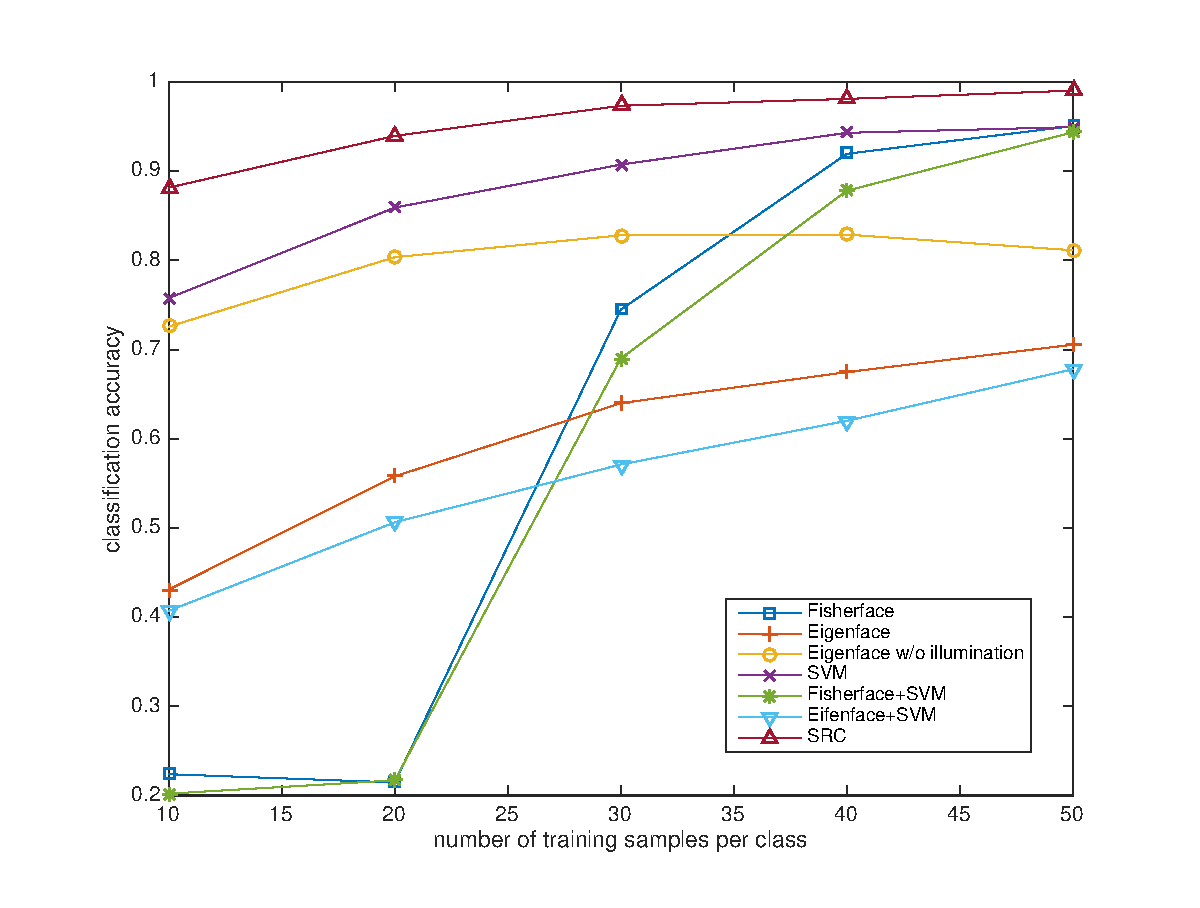
\includegraphics[width=0.5\textwidth]{inftr}
	\caption{Influence of training set size.}
	\label{inftr}
\end{figure}
First thing to notice is that when the size of training set is relatively small, the result of Fisherface, no matter with NN or SVM classifier is much worse even than guess. However, as the number of training sample increases, the classification accuracy increases sharply.

Applying SVM after Eigenface does not do any help to the result, instead, it even worse the situation as discussed above. Removing the largest three principal components in Eigenface results in a increase over all choice of training samples size, which verifies our deduction that by removing the principal components that capture illumination changes, the data is better clustered. The curve of Eigenface with out largest three principal components shows a decrease between 40 and 50, which is also mentioned in \cite{belhumeur1997eigenfaces}.

SRC and SVM shows top-level results over all choice of size, they are really reliable classifiers, however again the computational complexity involved in training the model is an issue that need to look into.

\section{Conclusion}
In this paper we explored four popular face recognition techniques, briefly introduced their theories, discussed their highlights as well as drawbacks. We did experiment to test the performance of them and some combinations of them. The experiment results shows that SRC outperformed other techniques without any fancy adjustments on parameters or strategies. Thus we can conclude that SRC is really a powerful and promising technique for the face recognition task, however further study might be needed to deal with the issue of computation.


% conference papers do not normally have an appendix


% use section* for acknowledgment

\bibliography{refs}
\bibliographystyle{unsrt}
\end{document}


